

\documentclass[a4paper]{article}
\usepackage{vntex}
%\usepackage[english,vietnam]{babel}
\usepackage[utf8]{inputenc}
%\usepackage[utf8]{inputenc}
%\usepackage[francais]{babel}
\usepackage{a4wide,amssymb,epsfig,latexsym,array,hhline,fancyhdr}
\usepackage[normalem]{ulem}
%\usepackage{soul}
\usepackage[makeroom]{cancel}
\usepackage{amsmath}
\usepackage{amsthm}
\usepackage{multicol,longtable,amscd}
\usepackage{diagbox}%Make diagonal lines in tables
\usepackage{booktabs}
\usepackage{alltt}
\usepackage{caption,subcaption}
\usepackage{lastpage}
\usepackage[lined,boxed,commentsnumbered]{algorithm2e}
\usepackage{enumerate}
\usepackage{graphicx}							% Standard graphics package
\usepackage{array}
\usepackage{multirow}
\usepackage{multicol}
\usepackage{rotating}
\usepackage{graphics}
\usepackage{geometry}
% \usepackage{hyperref}
\usepackage{setspace}
\usepackage{epsfig}
\usepackage{tikz}
\usepackage{listings}
\usepackage{color}
\usepackage{float}
\definecolor{barbiepink}{rgb}{0.85,0.09,0.52}
\definecolor{blackcoffee}{rgb}{0.23,0.18,0.18}
\definecolor{cgreen}{rgb}{0,0.6,0}
\definecolor{cgray}{rgb}{0.5,0.5,0.5}
\definecolor{cpurple}{rgb}{0.58,0,0.82}
\definecolor{backcolour}{rgb}{0.95,0.95,0.92}	
\usetikzlibrary{arrows,snakes,backgrounds}
\usepackage[unicode]{hyperref}
\lstset{
  breaklines=true,
  xleftmargin=15pt,
  xrightmargin=15pt,
  aboveskip=5pt,
  belowskip=5pt,
  backgroundcolor=\color{white},
  showstringspaces=false,
  frame=ltrb,
  language=python,
  tabsize=2,
  numbers=left,
  numberstyle=\small,
  numbersep=8pt,
  morekeywords={*, cos, sum, sin, np, pygame},
  commentstyle=\color{cgreen},
  keywordstyle=\color{magenta},
  numberstyle=\tiny\color{cgray},
  stringstyle=\color{cpurple},
  basicstyle=\ttfamily\footnotesize,
}

\def\thesislayout{	% A4: 210 × 297
	\geometry{
		a4paper,
		total={160mm,240mm},  % fix over page
		left=30mm,
		top=30mm,
	}
}


%\usepackage{fancyhdr}
\setlength{\headheight}{40pt}
\setlength{\parindent}{4pt}
\pagestyle{fancy}
\fancyhead{} % clear all header fields
\fancyhead[L]{
 \begin{tabular}{rl}
    \begin{picture}(25,15)(0,0)
    \put(0,-8){
\includegraphics[width=8mm, height=8mm]{Images/hcmut.png}}
    %\put(0,-8){\epsfig{width=10mm,figure=hcmut.eps}}
   \end{picture}&
	%
\includegraphics[width=8mm, height=8mm]{hcmut.png} & %
	\begin{tabular}{l}
		\textbf{\bf \ttfamily Trường Đại Học Bách Khoa Tp.Hồ Chí Minh}\\
		\textbf{\bf \ttfamily Khoa Điện-Điện tử}
	\end{tabular} 	
 \end{tabular}
}
\fancyhead[R]{
	\begin{tabular}{l}
		 \bf \\
		\bf 
	\end{tabular}  }
\fancyfoot{} % clear all footer fields
\fancyfoot[L]{\scriptsize \ttfamily Bài tập lớn môn Kỹ thuật Robot (EE3065) - HK241}
\fancyfoot[R]{\scriptsize \ttfamily Trang {\thepage}/\pageref{LastPage}}
\renewcommand{\headrulewidth}{0.3pt}
\renewcommand{\footrulewidth}{0.3pt}


%%%



\sloppy
\captionsetup[figure]{labelfont={small,bf},textfont={small,it},belowskip=-1pt,aboveskip=7pt}
\captionsetup[table]{labelfont={small,bf},textfont={small,it},belowskip=-1pt,aboveskip=7pt}
\setlength{\floatsep}{5pt plus 2pt minus 2pt}
\setlength{\textfloatsep}{5pt plus 2pt minus 2pt}
\setlength{\intextsep}{10pt plus 2pt minus 2pt}

\thesislayout
\renewcommand{\baselinestretch}{1.5}
\begin{document}
\large
\begin{titlepage}
\begin{center}
\textbf{\large ĐẠI HỌC QUỐC GIA THÀNH PHỐ HỒ CHÍ MINH} \\
\textbf{\large TRƯỜNG ĐẠI HỌC BÁCH KHOA} \\
\textbf{\large KHOA ĐIỆN-ĐIỆN TỬ} \\
\textbf{\large BỘ MÔN TỰ ĐỘNG} 
\end{center}
\begin{figure}[h!]
\begin{center}

\includegraphics[width=7cm]{Images/hcmut.png}
\end{center}
\end{figure}

\vspace{1cm}
\begin{center}
\begin{tabular}{c}
{\textbf{{\Large KỸ THUẬT ROBOT - EE3065}}}\\
~~\\
\hline
\\
\textbf{\large BÁO CÁO BÀI TẬP LỚN} \\
\textbf{\LARGE ARTICULATED ARM ROBOT} \\
\\
\hline
\end{tabular}
\end{center}

\vspace{1cm}

\begin{table}[h]
\begin{tabular}{rrlr}
\hspace{5 cm} & \large GVHD: & \large NGUYỄN HOÀNG GIÁP\\

& \large SV thực hiện: & \large HOÀNG SỸ NHẤT \\
& \large MSSV: & \large 2111915 \\

\end{tabular}
\end{table}
\vspace{2cm}
\begin{center}
{\bf Thành phố Hồ Chí Minh, Tháng 12/2024}
\end{center}
\end{titlepage}


%\thispagestyle{empty}

\newpage
\tableofcontents
\newpage
\section{GIỚI THIỆU}
\subsection{Sơ lược về Articulated Arm Robot}
Theo Robotic Institute of America (\textit{RIA}): Robot là một hệ thống đa tác vụ có thể lập trình được thiết kế để di chuyển vật liệu, bộ phận, dụng cụ hoặc thiết bị chuyên dụng thông qua chuyển động được lập trình theo các biến số để thực hiện các nhiệm vụ cụ thể đó, ngoài ra còn có thể thu thập thông tin từ môi trường và di chuyển thông minh theo đáp ứng.

Nhìn chung, “\textit{Robotic}” là thuật ngữ khoa học để định nghĩa lĩnh vực nghiên cứu khoa học về sự kết nối thông minh giữa việc ra quyết định và hành động. Do đó, có thể nhận định Robot là một chủ đề liên ngành liên quan đến các lĩnh vực cơ khí, điều khiển, máy tính và điện tử.

Articulated Arm là một loại cánh tay robot được thiết kế để mô phỏng chuyển động của cánh tay con người. Dưới đây là một số điểm nổi bật của Articulated Arm:
\begin{itemize}
    \item \textbf{Cấu trúc:}
    \begin{itemize}
        \item Gồm nhiều khâu (\textit{link}) được kết nối bằng các khớp (\textit{joint}).
        \item Các khớp có thể là khớp quay (\textit{cho phép xoay}) hoặc khớp dịch chuyển (\textit{cho phép di chuyển tuyến tính}).
    \end{itemize}
    \item \textbf{Bậc tự do:}
    \begin{itemize}
        \item Thường có nhiều bậc tự do, cho phép thực hiện các chuyển động và định vị phức tạp.
    \end{itemize}
    \item \textbf{End Effectors (\textit{Công cụ cuối}):}
    \begin{itemize}
        \item Có thể được trang bị nhiều công cụ hoặc kẹp ở cuối để thực hiện các nhiệm vụ cụ thể, như hàn, sơn, hoặc nhặt và đặt đồ vật.
    \end{itemize}
    \item \textbf{Hệ thống điều khiển:}
    \begin{itemize}
        \item Thường được điều khiển bởi các thuật toán và phần mềm tinh vi, cho phép thực hiện các chuyển động chính xác và tự động hóa.
    \end{itemize}
\end{itemize}

Articulated Arm được ứng dụng phổ biến trong các lĩnh vực:
\begin{itemize}
    \item \textbf{Sản xuất:} Được sử dụng rộng rãi trong dây chuyền lắp ráp cho các nhiệm vụ như hàn, sơn và đóng gói.
    \item \textbf{Chăm sóc sức khỏe:} Sử dụng trong các robot phẫu thuật để hỗ trợ bác sĩ trong các nhiệm vụ chính xác.
    \item \textbf{Nghiên cứu và phát triển:} Được sử dụng trong các phòng thí nghiệm cho các thí nghiệm yêu cầu thao tác chính xác với các đối tượng.
    \item \textbf{Giải trí:} Được sử dụng trong animatronics và hiệu ứng đặc biệt trong phim.
\end{itemize}

\begin{figure}[H]
    \centering
    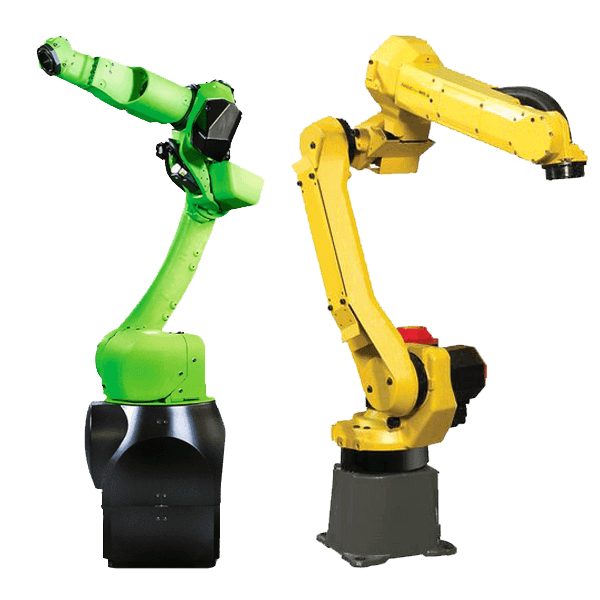
\includegraphics[width=0.75\linewidth]{Images/6-axis-duo.png}
    \caption{Các mẫu cánh tay robot trong công nghiệp}
    \label{fig:enter-label}
\end{figure}

\subsection{Giới thiệu về ngôn ngữ lập trình Python}
Python là một ngôn ngữ lập trình bậc cao, được phát triển bởi Guido van Rossum và lần đầu tiên được phát hành vào năm 1991. Nó nổi bật với cú pháp rõ ràng, dễ đọc và dễ học, giúp lập trình viên có thể phát triển ứng dụng một cách nhanh chóng và hiệu quả.

Các đặc điểm nổi bật của Python:
\begin{itemize}
    \item \textbf{Cú pháp đơn giản:}
    \begin{itemize}
        \item Python có cú pháp gần gũi với ngôn ngữ tự nhiên, giúp người mới bắt đầu dễ dàng tiếp cận.
    \end{itemize}
    \item \textbf{Đa năng:}
    \begin{itemize}
        \item Python có thể được sử dụng cho nhiều mục đích khác nhau, bao gồm phát triển web, phân tích dữ liệu, học máy, trí tuệ nhân tạo, tự động hóa, và nhiều lĩnh vực khác.
    \end{itemize}
    \item \textbf{Thư viện phong phú:}
    \begin{itemize}
        \item Python có một hệ sinh thái thư viện phong phú, bao gồm các thư viện nổi tiếng như NumPy, Pandas, Matplotlib, TensorFlow và Django, giúp lập trình viên dễ dàng thực hiện các tác vụ phức tạp.
    \end{itemize}
    \item \textbf{Hỗ trợ lập trình hướng đối tượng:}
    \begin{itemize}
        \item Python hỗ trợ lập trình hướng đối tượng, cho phép người lập trình tổ chức mã nguồn một cách hiệu quả hơn.
    \end{itemize}
    \item \textbf{Cộng đồng lớn:}
    \begin{itemize}
        \item Python có một cộng đồng lập trình viên lớn và năng động, cung cấp nhiều tài nguyên, hướng dẫn và hỗ trợ.
    \end{itemize}
\end{itemize}

Trong bài tập lớn này sẽ sử dụng Python và các thư viện hỗ trợ sau sau để tạo giao diện và giả lập cánh tay robot:
\begin{itemize}
    \item \textbf{Pygame:}
    \begin{itemize}
        \item Thư viên dùng để vẽ 2-D và tạo animation cũng như tương tác với bàn phím để xoay góc nhìn trong môi trường giả lập cánh tay robot.
    \end{itemize}
    \item \textbf{Numpy:}
    \begin{itemize}
        \item Thư viện Numpy được sử dụng để tính toán các ma trận và một vài phép toán học cơ bản.
    \end{itemize}
    \item \textbf{Matplotlib:}
    \begin{itemize}
        \item Dùng để vẽ đồ thị.
    \end{itemize}
    \item \textbf{Tkinter:}
    \begin{itemize}
        \item Thư viện hỗ trợ tạo giao diện người dùng UI \textit{(User Interface}).
    \end{itemize}
\end{itemize}
\begin{figure}[H]
	\centering
	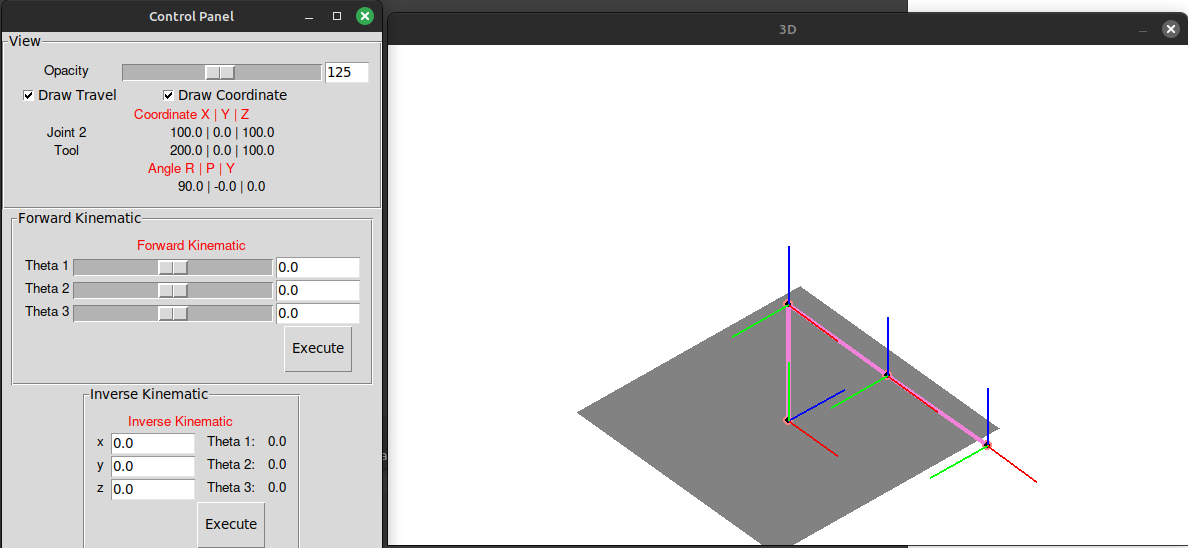
\includegraphics[width=1\linewidth]{Images/software.png}
	\caption{Chương trình được viết bằng Python}
	\label{fig:enter-label1}
\end{figure}
\newpage
\section{ĐỘNG HỌC THUẬN}
\subsection{DH-Table}
\newpage
\section{ĐỘNG HỌC NGHỊCH}
\subsection{Lập công thức giải bài toán động học nghịch}

\subsection{Xây dựng UI và Animation cho bài toán động lực nghịch}
\subsubsection{Giao điện người dùng UI}

Xây dựng giao diện để người dùng nhập tọa độ vị trí của End effector, sau khi bấm nút \textit{Execute} robot sẽ tiến hành di chuyển đến vị trí trên.

\begin{figure}[H]
	\centering
	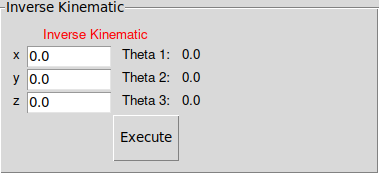
\includegraphics[width=1\linewidth]{Images/inv_ui.png}
	\caption{Giao diện Inverse Kinematic}
	\label{fig:enter-label8}
\end{figure}

\subsubsection{Tạo animation và di chuyển robot theo bài toán động lực nghịch}

Dựa vào các công thức đã lập được ở trên và các giá trị $x$, $y$ và $z$ do người dùng nhập ta tính ngược lại giá trị các góc $\theta_{1}$ , $\theta_{2}$ và $\theta_{3}$, sau khi kiểm tra các góc xaoy có nằm trong phạm vi giới hạn quya của từng khớp ta tiến hành cho robot chuyển động giống như bài toán thuận theo các giá trị $\theta$ vừa tính được ở trên.

\vspace{0.5cm}
\begin{lstlisting}[language=python]
	def inverseKine():
	global guiThetaInv
	px = guiCoorInv[0].get()
	py = guiCoorInv[1].get()
	pz = guiCoorInv[2].get()-d[0]
	# Check valid
	valid = 0
	tmp = (px**2+py**2+pz**2)**0.5
	if (tmp <= a[1]+a[2]) and (tmp >= abs(a[1]-a[2])) and (pz+d[0] >= 0): 
	# calculate
	c3 = (px**2+py**2+pz**2-a[1]**2-a[2]**2)/(2*a[1]*a[2])
	s3 = (1-c3**2)**0.5
	theta3 = atan2(s3, c3)
	
	theta2 = atan2(pz, (px**2+py**2)**0.5) - acos((px**2+py**2+pz**2+a[1]**2-a[2]**2)/(2*a[1]*(px**2+py**2+pz**2)**0.5))
	
	theta1 = atan2(py, px)
	
	valid = 1
	for i, thetaN in enumerate([theta1, theta2, theta3]):
	if thetaN < limitTheta[i][0] or thetaN > limitTheta[i][1]:
	valid = 0
	else: guiThetaInv[i].set(round(thetaN*180/pi, 3))
	
	if valid:
	deltaTime = 60
	nextTheta = np.array([theta1, theta2, theta3])
	stepAngle = np.array([(nextTheta[0]-theta[0])/deltaTime, (nextTheta[1]-theta[1])/deltaTime, (nextTheta[2]-theta[2])/deltaTime])
	animateTranform(nextTheta, stepAngle, deltaTime)
	else:
	tkinter.messagebox.showwarning("Inverse Kinematic.",  "Out of workspace")
\end{lstlisting}

\begin{figure}[H]
	\centering
	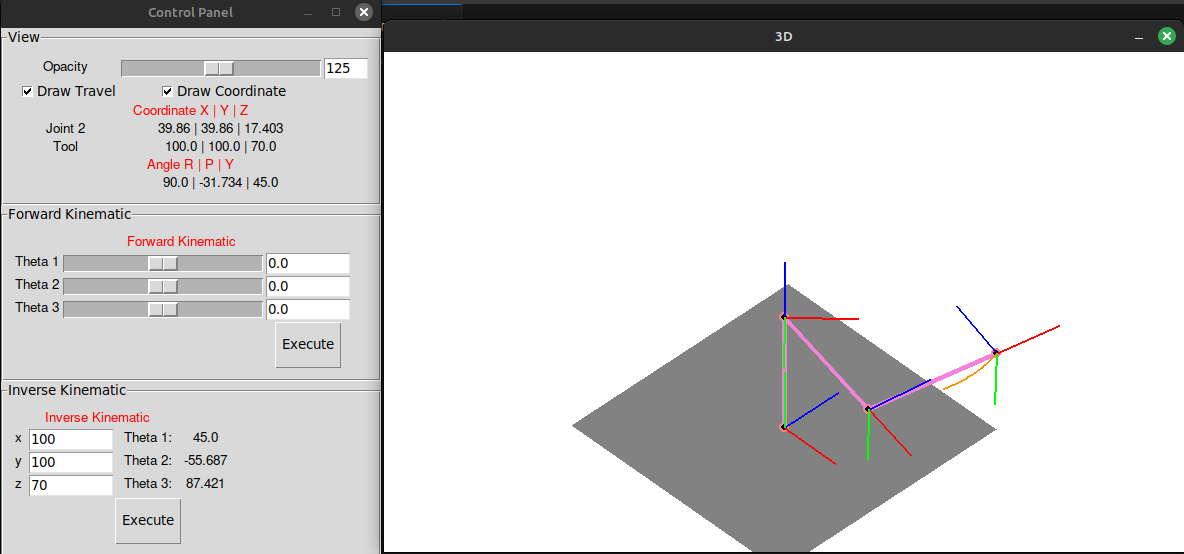
\includegraphics[width=1\linewidth]{Images/inv_demo.png}
	\caption{Inverse Kinematic}
	\label{fig:enter-label9}
\end{figure}
\newpage
\section{QUY HOẠCH QUỸ ĐẠO TRAJECTORY PLANNING}
\subsection{DH-Table}
\newpage
\section{MA TRẬN JACOBI VÀ ĐIỂM KÌ DỊ}
\subsection{DH-Table}
\newpage
\section{Path Finding}
\subsection{Sơ lược về bài toán}
Bài toán Path Finding là một trong những bài toán cơ bản trong lĩnh vực Trí tuệ Nhân tạo, với mục tiêu tìm đường đi ngắn nhất từ một điểm khởi đầu (\textit{start}) đến một điểm kết thúc (\textit{goal}) trên một bản đồ hoặc đồ thị. 

Giải thuật A* (\textit{A-star}) được lựa chọn để giải quyết bài toán này nhờ vào tính hiệu quả cao trong việc kết hợp giữa hai phương pháp: tìm kiếm tham lam (\textit{Greedy Search}) và tìm kiếm chi phí đều (\textit{Uniform Cost Search}). Giải thuật này sử dụng công thức:
\[
f(n) = g(n) + h(n)
\]
Trong đó:
\begin{itemize}
    \item $f(n)$: Hàm lượng giá tổng hợp.
    \item $g(n)$: Chi phí từ điểm bắt đầu đến trạng thái $n$.
    \item $h(n)$: Heuristic (ước lượng chi phí từ trạng thái $n$ đến đích).
\end{itemize}

Trong bài toán này, nhóm lựa chọn sẽ áp dụng giải thuật A* để tìm đường đi ngắn nhất từ điểm bắt đầu đến điểm đích trên một bản đồ lưới 2D.


\subsection{Những đánh giá về game}
Path Finding là một bài toán không chỉ mang tính thực tiễn cao mà còn chứa đựng nhiều khía cạnh học thuật quan trọng trong lĩnh vực Trí tuệ Nhân tạo. Đây là nền tảng của nhiều ứng dụng thực tế như:
\begin{itemize}
    \item Định tuyến trong giao thông vận tải, các ứng dụng bản đồ.
    \item Điều hướng cho các nhân vật trong các trò chơi điện tử.
    \item Điều hướng robot trong lĩnh vực Robotics.
\end{itemize}
Tuy nhiên, việc giải quyết bài toán này có thể bị ảnh hưởng bởi độ lớn của không gian trạng thái, độ phức tạp của các phép di chuyển, và chất lượng của hàm lượng giá. Một heuristic không phù hợp có thể dẫn đến kết quả kém tối ưu, hoặc khiến thuật toán phải duyệt qua quá nhiều trạng thái.

Giải thuật A* với cơ chế tối ưu hoá chi phí bằng cách kết hợp hàm $g(n)$ (chi phí đã đi) và hàm $h(n)$ (ước lượng chi phí còn lại) là một giải pháp mạnh mẽ. Việc đánh giá và cải thiện heuristic phù hợp là yếu tố then chốt trong việc nâng cao hiệu quả của thuật toán.

\subsection{Giao diện trực quan hóa}
Để trực quan hóa kết quả của thuật toán A*, nhóm em đã xây dựng một giao diện minh họa bằng Python, sử dụng thư viện \texttt{matplotlib} để vẽ bản đồ và đường đi. Dưới đây là chi tiết về cách thức hoạt động của giao diện:

\begin{itemize}
    \item Mỗi ô trên bản đồ được hiển thị bằng một màu sắc khác nhau, tương ứng với các trạng thái:
    \begin{itemize}
        \item \textbf{0: Passage (đường đi trống)} - màu đen.
        \item \textbf{1: Wall (vật cản)} - màu tím đậm.
        \item \textbf{2: Start (điểm bắt đầu)} - màu đỏ.
        \item \textbf{3: Destination (điểm đích)} - màu cam.
        \item \textbf{4: Path (đường đi tìm được)} - màu vàng nhạt.
    \end{itemize}
    \item Giao diện có thể tạo tùy chỉnh một bản đồ kích thước \( width \times height \), với tỷ lệ vật cản \textit{wallrate}. Với điểm bắt đầu và điểm đích nếu không được tùy chỉnh thì sẽ được sinh ngẫu nhiên.
    \item Các đường đi được vẽ bằng cách tô màu các ô thuộc đường đi ngắn nhất từ điểm bắt đầu đến điểm đích.
\end{itemize}



\newpage
Dưới đây là một vài kết quả trực quan hóa:

\begin{figure}[H]
    \centering
    \includegraphics[width=0.8\textwidth]{Images/pathfinding/output.png}
    \caption{Kết quả trực quan cho bản đồ có kích thước 20x20, tỉ lệ vật cản là 0.3.}
    \label{fig:visualization1}
\end{figure}

\begin{figure}[H]
    \centering
    \includegraphics[width=0.8\textwidth]{Images/pathfinding/output2.png}
    \caption{Kết quả trực quan cho bản đồ có kích thước 10x10, tỉ lệ vật cản là 0.3.}
    \label{fig:visualization2}
\end{figure}
\newpage
\subsection{Xây dựng các cấu trúc để mô phỏng bài toán}
Ở trò chơi này, nhóm em tổ chức các đoạn mã Python trên các tệp tin gồm Map.py, Astar.py, visualize.ipynb và có một file map1.txt dành cho trường hợp muốn tùy chỉnh sâu cấu trúc bản đồ lưới 2D:
Để giải quyết bài toán tìm đường (Path Finding) bằng giải thuật A*, nhóm em đã triển khai hai file Python chính là \texttt{astar.py} và \texttt{map.py}. 

\subsubsection{Cấu trúc file \texttt{astar.py}}
\begin{lstlisting}[language=python, caption=Định nghĩa các lớp trong file astar.py]
class Cell:
    def __init__(self):
class AStart:
    def __init__(self, map, movedir=4):
    def Search(self):
    def PrintPath(self):
    def UpdateGrid(self):
\end{lstlisting}

\textbf{Giải thích:}
\begin{itemize}
    \item \texttt{class Cell}: Đại diện cho từng ô trong bản đồ.
    \begin{itemize}
        \item Thuộc tính:
        \begin{itemize}
            \item \texttt{parent\_x, parent\_y}: Tọa độ của ô cha.
            \item \texttt{f, g, h}: Các giá trị tổng chi phí, chi phí đến ô, và ước lượng đến đích.
        \end{itemize}
    \end{itemize}
    \item \texttt{class AStart}: Thực hiện thuật toán A*.
    \begin{itemize}
        \item Phương thức:
        \begin{itemize}
            \item \texttt{Search}: Triển khai thuật toán A* để tìm đường đi.
            \item \texttt{PrintPath}: In đường đi từ điểm đầu đến điểm đích.
            \item \texttt{UpdateGrid}: Cập nhật bản đồ với đường đi tìm được.
        \end{itemize}
    \end{itemize}
\end{itemize}

\subsubsection{Cấu trúc file \texttt{map.py}}
\begin{lstlisting}[language=python, caption=Định nghĩa các lớp trong file map.py]
class Map:
    def CreateWall(self, wall_rate=0.3):
    def IsValid(self, x, y):
    def IsBlock(self, x, y):
    def CalculateH(self, x, y, algorithm):
\end{lstlisting}

\textbf{Giải thích:}
\begin{itemize}
    \item \texttt{class Map}: Đại diện cho bản đồ trong bài toán.
    \begin{itemize}
        \item \textbf{Thuộc tính}:
        \begin{itemize}
            \item \texttt{width, height}: Kích thước bản đồ.
            \item \texttt{grid}: Ma trận biểu diễn bản đồ.
            \item \texttt{src\_point, des\_point}: Tọa độ điểm bắt đầu và điểm kết thúc.
        \end{itemize}
        \item \textbf{Phương thức}:
        \begin{itemize}
            \item \texttt{CreateWall}: Tạo các vật cản ngẫu nhiên trên bản đồ.
            \item \texttt{IsValid}: Kiểm tra xem tọa độ có hợp lệ không.
            \item \texttt{IsBlock}: Kiểm tra xem tọa độ có bị chặn bởi vật cản (tường) không.
            \item \texttt{IsDestination}: Kiểm tra xem tọa độ có phải điểm đích không.
            \item \texttt{CalculateH}: Tính toán heuristic theo thuật toán Manhattan hoặc Euclidean.
        \end{itemize}
    \end{itemize}
\end{itemize}
\subsection{Định nghĩa không gian trạng thái}

Trong bài toán Path Finding, không gian trạng thái được định nghĩa như sau:

\begin{itemize}
    \item \textbf{Trạng thái:} 
    Mỗi trạng thái trong không gian trạng thái là một tọa độ $(x, y)$ trên bản đồ lưới 2D kích thước $n \times m$, trong đó:
    \begin{itemize}
        \item $x$: Chỉ số hàng (row index).
        \item $y$: Chỉ số cột (column index).
    \end{itemize}
    
    \item \textbf{Trạng thái khởi đầu (Start State):} 
    Là tọa độ ban đầu $S = (x_s, y_s)$, nơi bắt đầu tìm kiếm đường đi.

    \item \textbf{Trạng thái kết thúc (Goal State):} 
    Là tọa độ đích $G = (x_g, y_g)$, nơi cần tìm đến.

    \item \textbf{Trạng thái cản trở (Obstacle):} 
    Các ô không thể đi qua được trên bản đồ, ký hiệu là $W$ (Wall).

    \item \textbf{Trạng thái trung gian (Intermediate State):}
    Các ô có thể đi qua trong quá trình tìm kiếm, ký hiệu là $P$ (Passage).
\end{itemize}

\textbf{Không gian trạng thái:} 
Không gian trạng thái là tập hợp tất cả các tọa độ $(x, y)$ khả thi trên bản đồ, được định nghĩa là:
\[
\mathcal{S} = \{(x, y) \ | \ 0 \leq x < n, 0 \leq y < m, (x, y) \notin W \}
\]

\textbf{Hàm chuyển trạng thái (State Transition Function):} 
Các trạng thái chuyển đổi được định nghĩa bởi các quy tắc di chuyển:
\begin{itemize}
    \item Di chuyển sang trái: $(x, y) \rightarrow (x, y-1)$
    \item Di chuyển sang phải: $(x, y) \rightarrow (x, y+1)$
    \item Di chuyển lên: $(x, y) \rightarrow (x-1, y)$
    \item Di chuyển xuống: $(x, y) \rightarrow (x+1, y)$
\end{itemize}

Các phép di chuyển này chỉ khả thi nếu tọa độ mới $(x', y')$ thỏa mãn:
\[
(x', y') \in \mathcal{S}.
\]

\textbf{Hàm lượng giá (Heuristic Function):} 
Để tối ưu hóa quá trình tìm kiếm, nhóm em sử dụng hàm lượng giá $h(n)$ để ước lượng chi phí từ trạng thái hiện tại đến trạng thái đích:

\textbf{Manhattan Distance:} 
\[
h(x, y) = |x - x_g| + |y - y_g|
\] 
Ngoài ra để mở rộng bài toán cho trường hợp Agent di chuyển được cả hướng chéo thì sẽ dùng hàm lượng giá:

\textbf{Euclidean Distance:} 
\[
h(x, y) = \sqrt{(x - x_g)^2 + (y - y_g)^2}
\]


Với định nghĩa trên, không gian trạng thái và các phép chuyển đổi đã được thiết lập để áp dụng giải thuật A*.
 


\subsection{A*  Search}
\begin{itemize}
    \item \textbf{Pseudocode:}\\
    Thuật toán A* được triển khai như sau:

function AStarSearch(start, goal, map):\\
    1. Khởi tạo danh sách mở (Open List) chứa ô bắt đầu, với f = 0.\\
    2. Khởi tạo danh sách đóng (Closed List) rỗng.\\
    While Open List không rỗng:\\
        3. Lấy ô trong danh sách mở có f nhỏ nhất làm ô hiện tại.\\
        4. Nếu ô hiện tại là đích, dừng thuật toán và trả về đường đi.\\
        5. Duyệt qua các ô lân cận của ô hiện tại:\\
            a. Nếu ô không hợp lệ hoặc là vật cản, bỏ qua.\\
            b. Nếu ô đã được xét trong danh sách đóng, bỏ qua.\\
            c. Tính giá trị g, h, và f cho ô lân cận:\\
                - g = chi phí từ điểm bắt đầu đến ô lân cận.\\
                - h = ước lượng chi phí từ ô lân cận đến đích(heuristic).\\
                - f = g + h.\\
            d. Nếu ô lân cận chưa có trong danh sách mở hoặc có f nhỏ hơn, cập nhật danh sách mở.\\
        6. Thêm ô hiện tại vào danh sách đóng.\\
    7. Nếu danh sách mở rỗng nhưng chưa tìm được đích, trả về thất bại.\\




    \item \textbf{Áp dụng vào bài toán và kết quả:}\\
    Thuật toán A* được áp dụng để giải bài toán tìm đường trên bản đồ lưới \(20 \times 20\) với tỷ lệ vật cản là \(30\%\). 

    \begin{itemize}
        \item \textbf{Các bước chính:}
        \begin{enumerate}
            \item \textbf{Khởi tạo danh sách mở và danh sách đóng:} 
                  - Danh sách mở (\textit{Open List}) chứa các ô cần được xét.
                  - Danh sách đóng (\textit{Closed List}) chứa các ô đã xét.
            \item \textbf{Tính toán các giá trị \(f, g, h\):}
            
                  - \(g(n)\): Chi phí từ điểm bắt đầu đến ô hiện tại.\\
                  - \(h(n)\): Heuristic dựa trên khoảng cách Manhattan hoặc Euclidean.\\
                  - \(f(n) = g(n) + h(n)\).
            \item \textbf{Tìm ô có giá trị \(f\) nhỏ nhất:} 
                  Duyệt các ô xung quanh (theo 4 hoặc 8 hướng) và cập nhật danh sách mở.
            \item \textbf{Lưu lại đường đi tối ưu:} Truy xuất từ điểm đích ngược về điểm bắt đầu bằng cách sử dụng \texttt{parent\_x} và \texttt{parent\_y}.
        \end{enumerate}

        \item \textbf{Minh họa kết quả:}
        Sau khi áp dụng thuật toán, đường đi tối ưu được đánh dấu trên bản đồ với màu vàng.
        \begin{figure}[H]
            \centering
            \includegraphics[width=0.7\textwidth]{Images/pathfinding/output.png}
            \caption{Kết quả đường đi tìm được bằng thuật toán A*.}
            \label{fig:astar_result}
        \end{figure}

        \item \textbf{Đánh giá:}
        \begin{itemize}
            \item Thuật toán tìm được đường đi ngắn nhất với chi phí tối ưu.
            \item Áp dụng heuristic Manhattan giúp giảm số ô cần xét trong danh sách mở.
            \item Với bản đồ có kích thước lớn, bộ nhớ sử dụng cho danh sách mở và đóng có thể tăng đáng kể.
        \end{itemize}
    \end{itemize}
\end{itemize}

\newpage



\newpage
\section{ĐÁNH GIÁ CHUNG VÀ KẾT LUẬN}
Sau thời gian thực hiện bài tập lớn số 1 môn Nhập môn Trí tuệ nhân tạo, nhóm có những đánh giá và kết luận chung sau khi hoàn thành bài tập lớn này như sau :
\begin{itemize}
    \item Về những kết quả thu được:
    \begin{itemize}
        \item Biết cách mô phỏng bài toán cũng như kết quả dưới dạng các ứng dụng đơn giản trên nền tảng ngôn ngữ Python 3 bằng cách áp dụng linh hoạt các module cũng như sử dụng các framework hiệu quả.
        \item Hiểu được cấu trúc và những thành phần cơ bản của các bài toán để từ đó xây dựng được các cấu trúc để mô phỏng bài toán. 
        \item Đã hiểu rõ cũng như biết cách áp dụng 4 giải thuật tìm kiếm cơ bản đó là Depth-First Search, Genetic, A* Search  vào để tìm lời giải cho bài toán.
        \item Cải thiện được khả năng lập trình bằng ngôn ngữ Python 3, tận dụng các module sẵn có vô cùng hữu ích của ngôn ngữ này. 
        \item Nâng cao khả năng làm việc theo nhóm cũng như khả năng hoàn thành công việc độc lập và đúng thời gian của từng thành viên trong nhóm. 
    \end{itemize}
    \item Về những hạn chế còn tồn đọng:
    \begin{itemize}
        \item Cải thiện được khả năng lập trình bằng ngôn ngữ Python 3, tận dụng các module sẵn có vô cùng hữu ích của ngôn ngữ này.
    \end{itemize}
\end{itemize}
Qua những đánh giá và kết luận chung như trên, các thành viên của nhóm đều nhận thấy rằng bản thân đã học thêm được khá nhiều điều mới lạ và đã rèn dũa thêm được những kỹ năng sẵn có. Tuy vậy thì nhóm cũng nhận ra được vẫn còn khá nhiều khuyết điểm quan trọng cần được khắc phục ngay để có thể thực hiện những dự án khác trong tương lai một cách đầy đủ và hoàn thiện hơn. 
\section{VIDEO DEMO VÀ CODE PYTHON}
Link video thuyết trình: \href{}{Nền tảng Youtube}\\
Link slide thuyết trình: \href{}{Nền tảng Canva}
\addcontentsline{toc}{section}{Tài liệu}
\begin{thebibliography}{99999}

\end{thebibliography}
\end{document}
